% !TeX root = ../main.tex

\chapter{Results}\label{chapter:results}

\section{Overall EuRoC Results}

All reported configurations completed all eleven EuRoC sequences. The
full-sequence ATE and RTE-6 results are given in \autoref{tab:euroc-ate} and
\autoref{tab:euroc-rte6}. The VOCA columns use their frozen evaluations rather
than later instrumented diagnostic runs.

\begin{table}[p]
  \centering
  \caption[Absolute trajectory error on EuRoC]{Aligned absolute trajectory error (ATE) in metres on all EuRoC
  sequences. Lower is better; bold denotes the lowest value in a row.}
  \label{tab:euroc-ate}
  \begin{tabular}{@{}lrrrr@{}}
    \toprule
    Sequence & Stationary & PVO & VOCA MV-first & VOCA OF-first \\
    \midrule
    EMH01 & 4.308 & 0.246 & 0.172 & \textbf{0.118} \\
    EMH02 & 4.646 & 0.594 & 0.123 & \textbf{0.104} \\
    EMH03 & 3.580 & 1.082 & \textbf{0.200} & 0.212 \\
    EMH04 & 6.821 & 4.722 & 0.234 & \textbf{0.202} \\
    EMH05 & 6.879 & 4.089 & 0.228 & \textbf{0.181} \\
    EV101 & 1.853 & 0.226 & 0.101 & \textbf{0.096} \\
    EV102 & 1.778 & 0.514 & \textbf{0.074} & 0.085 \\
    EV103 & 1.574 & 12.565 & 0.513 & \textbf{0.438} \\
    EV201 & 2.299 & 0.935 & 0.267 & \textbf{0.090} \\
    EV202 & 2.111 & 2.087 & 0.137 & \textbf{0.104} \\
    EV203 & \textbf{1.959} & 6.497 & 9.532 & 2.508 \\
    \bottomrule
  \end{tabular}
\end{table}

\begin{table}[p]
  \centering
  \caption[Six-frame relative translation error on EuRoC]{Relative translation error over non-overlapping six-frame intervals
  (RTE-6), in metres. Lower is better; bold denotes the lowest value in a row.}
  \label{tab:euroc-rte6}
  \begin{tabular}{@{}lrrrr@{}}
    \toprule
    Sequence & Stationary & PVO & VOCA MV-first & VOCA OF-first \\
    \midrule
    EMH01 & 0.1573 & 0.0092 & \textbf{0.0063} & 0.0066 \\
    EMH02 & 0.1685 & 0.0123 & \textbf{0.0060} & 0.0061 \\
    EMH03 & 0.3659 & 0.0476 & 0.0150 & \textbf{0.0145} \\
    EMH04 & 0.3414 & 0.1344 & 0.0213 & \textbf{0.0196} \\
    EMH05 & 0.3149 & 0.1195 & \textbf{0.0159} & 0.0162 \\
    EV101 & 0.1365 & 0.0189 & 0.0142 & \textbf{0.0140} \\
    EV102 & 0.3037 & 0.0359 & 0.0163 & \textbf{0.0155} \\
    EV103 & 0.2536 & 2.0434 & \textbf{0.0618} & 0.0643 \\
    EV201 & 0.1084 & 0.0818 & 0.0551 & \textbf{0.0163} \\
    EV202 & 0.2441 & 0.2078 & 0.0167 & \textbf{0.0145} \\
    EV203 & 0.3296 & 0.5169 & 1.5336 & \textbf{0.2455} \\
    \bottomrule
  \end{tabular}
\end{table}

PVO improves on the stationary trajectory in both ATE and RTE-6 on nine of
eleven sequences. It therefore recovers camera motion over most of the benchmark,
but EV103 and EV203 show that the method is not consistently better than
predicting no motion. Its macro ATE is \SI{3.051}{\metre} and its median ATE is
\SI{1.082}{\metre}; its macro RTE-6 is \SI{0.2934}{\metre} and its median RTE-6
is \SI{0.0818}{\metre}. The gap between mean and median is dominated by the
EV103 outlier.

\begin{figure}[htbp]
  \centering
  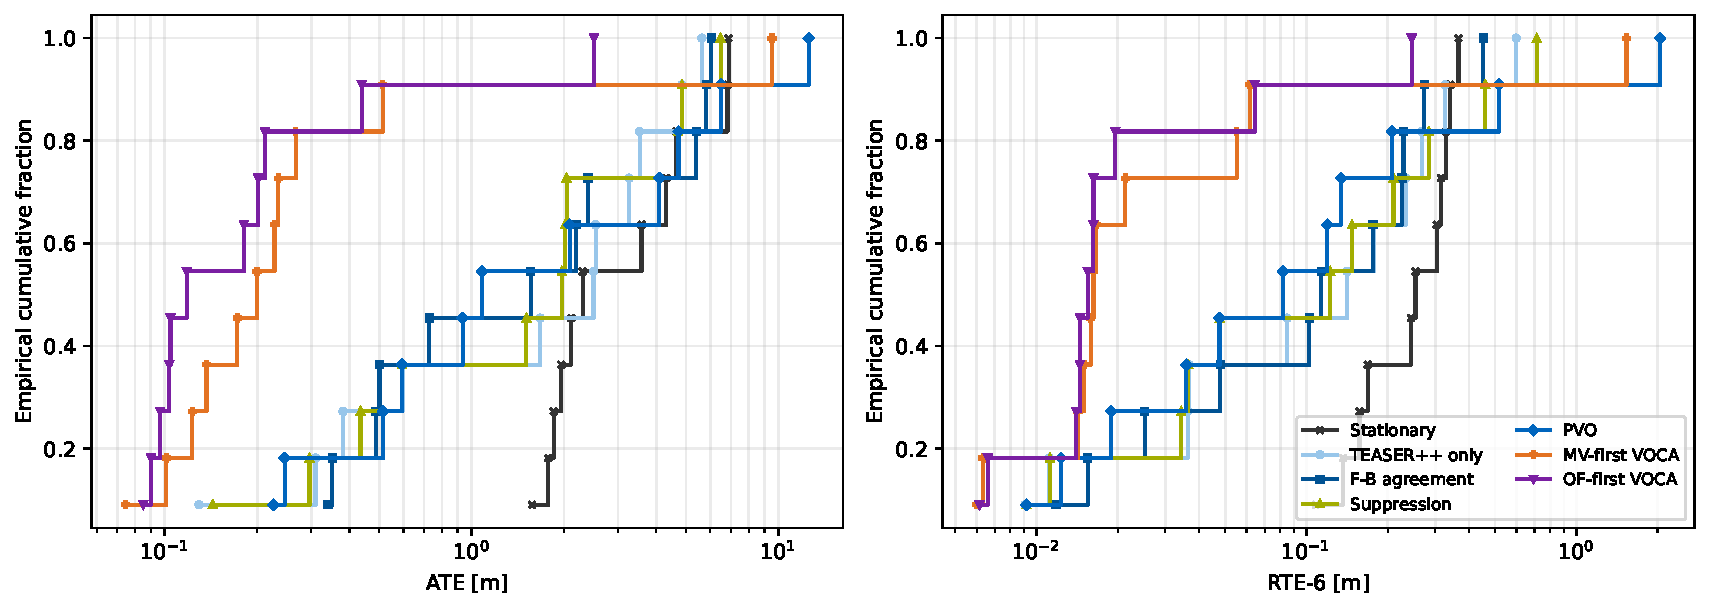
\includegraphics[width=\textwidth]{figures/evaluation/trajectory-error-ecdf}
  \caption[Distributions of full-sequence trajectory errors]{Empirical cumulative distributions over the eleven full-sequence ATE
  values (left) and RTE-6 values (right). The logarithmic horizontal axes retain
  the effect of both low-error sequences and large failures.}
  \label{fig:trajectory-error-ecdf}
\end{figure}

\subsection{Trajectory Geometry}\label{sec:trajectory-geometry}

The trajectory overlays illustrate the central feasibility result: motion
vectors alone can support reasonable camera-motion tracking.
The easy Machine Hall sequences give especially clear examples:
\autoref{fig:trajectory-emh01-separated} and
\autoref{fig:trajectory-emh02-separated} show close agreement with the
reference paths on EMH01 and EMH02. The medium EMH03 sequence and EV201
follow in \autoref{fig:trajectory-emh03-separated} and
\autoref{fig:trajectory-ev201-separated}. Their codec-only estimates recover
the broad shape of the reference route, with visible deviations in position
and vertical motion. Each method is shown separately against ground truth,
with common axes for comparison within a sequence.

These results demonstrate one way to recover useful trajectory geometry from
codec motion vectors and motivate further investigation of pixel-free VO.
Full-sequence PVO overlays for all eleven sequences, including failure cases,
are provided in \autoref{appendix:full-trajectories}; the temporal evidence for
failures is examined in \autoref{sec:failure-episodes}.

\begin{figure}[p]
  \centering
  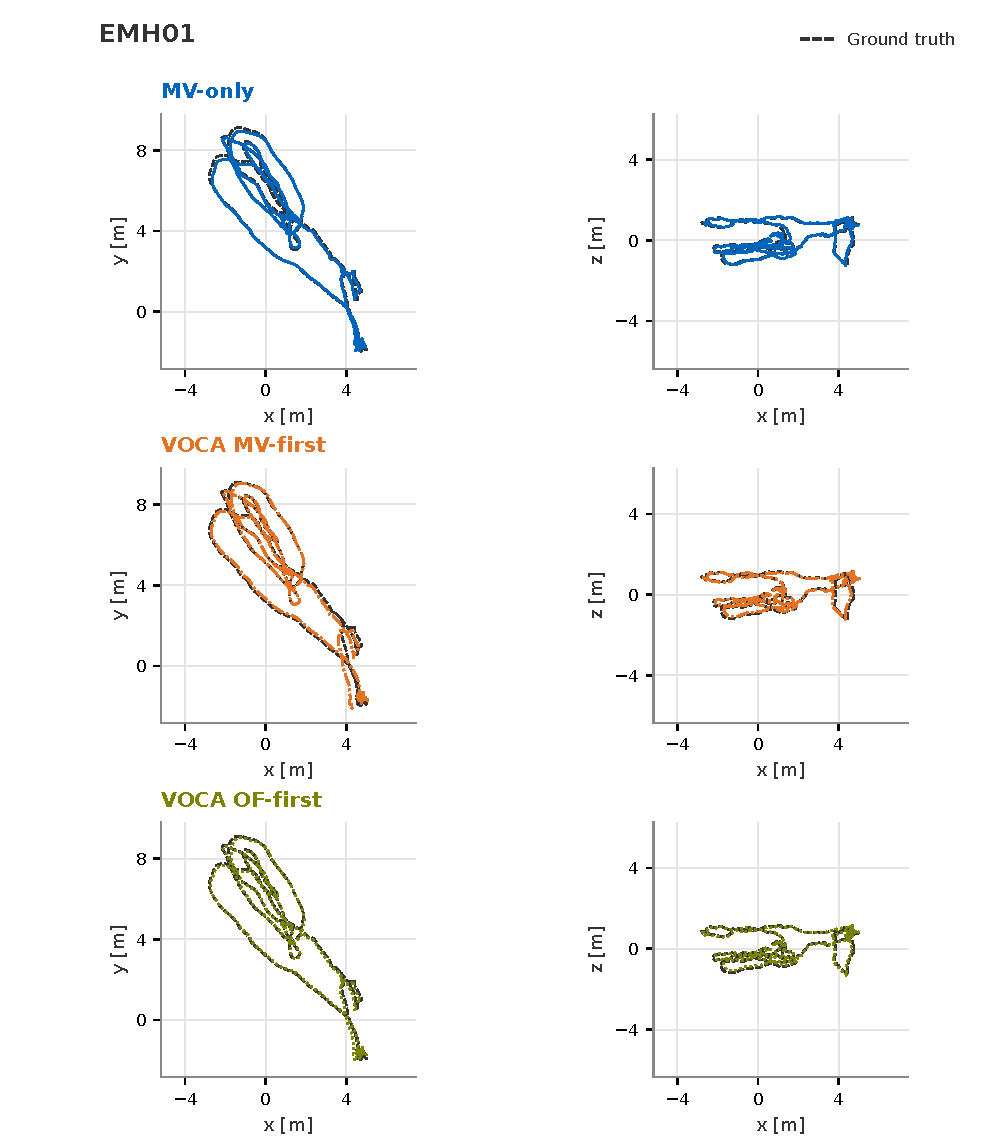
\includegraphics[width=\textwidth]{figures/evaluation/trajectory-emh01-separated.pdf}
  \caption[EMH01 trajectory comparison]{Full-sequence EMH01 trajectories. Top to bottom: MV-only,
  VOCA MV-first, and VOCA OF-first, each with ground truth. Left: $xy$;
  right: $xz$. All rows share the same spatial limits and metric scale.
  Each complete estimate uses its rigid alignment for ATE, shared between
  projections, without scale correction. All saved estimates are shown.}
  \label{fig:trajectory-emh01-separated}
\end{figure}

\begin{figure}[p]
  \centering
  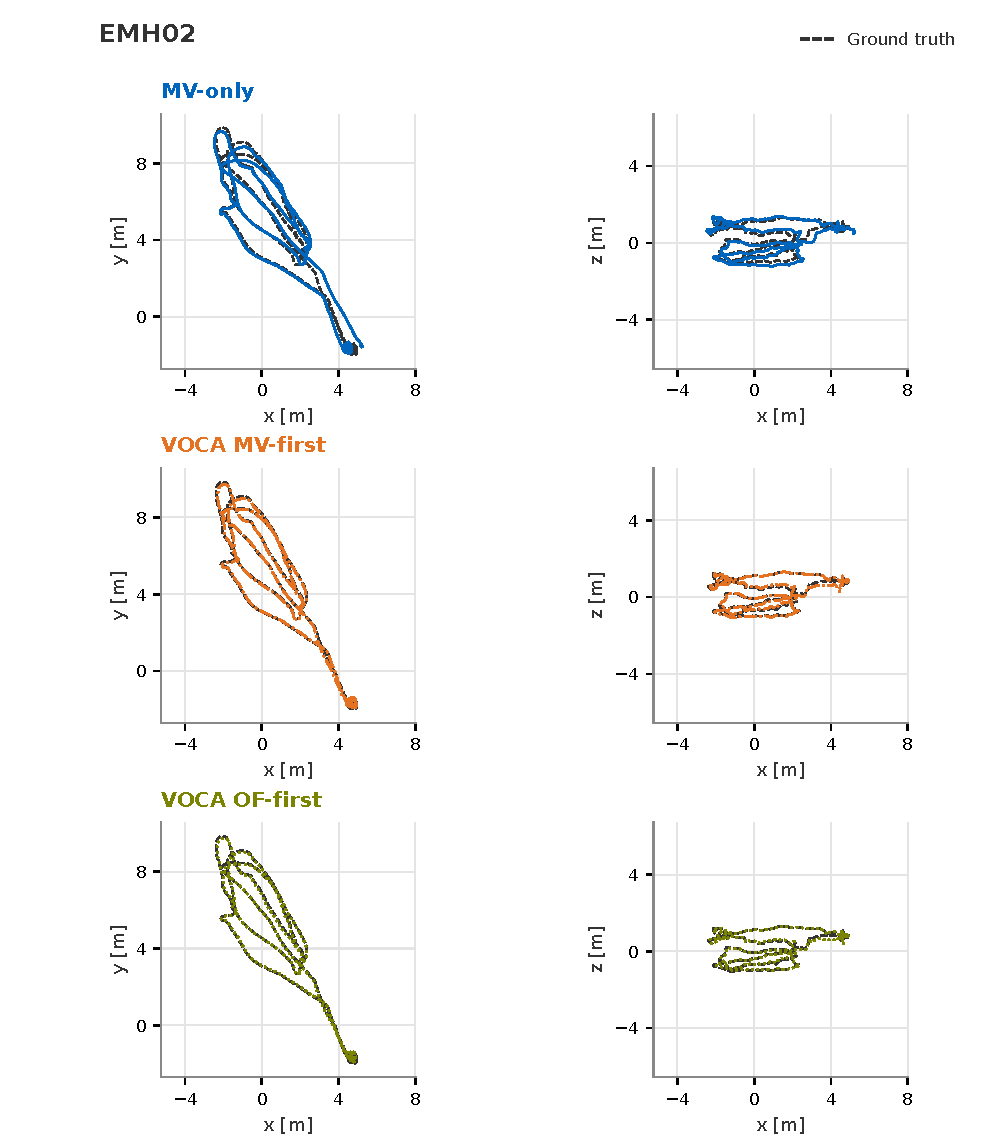
\includegraphics[width=\textwidth]{figures/evaluation/trajectory-emh02-separated.pdf}
  \caption[EMH02 trajectory comparison]{Full-sequence EMH02 trajectories. Top to bottom: MV-only,
  VOCA MV-first, and VOCA OF-first, each with ground truth. Left: $xy$;
  right: $xz$. Alignment and plotting conventions follow
  \autoref{fig:trajectory-emh01-separated}.}
  \label{fig:trajectory-emh02-separated}
\end{figure}

\begin{figure}[p]
  \centering
  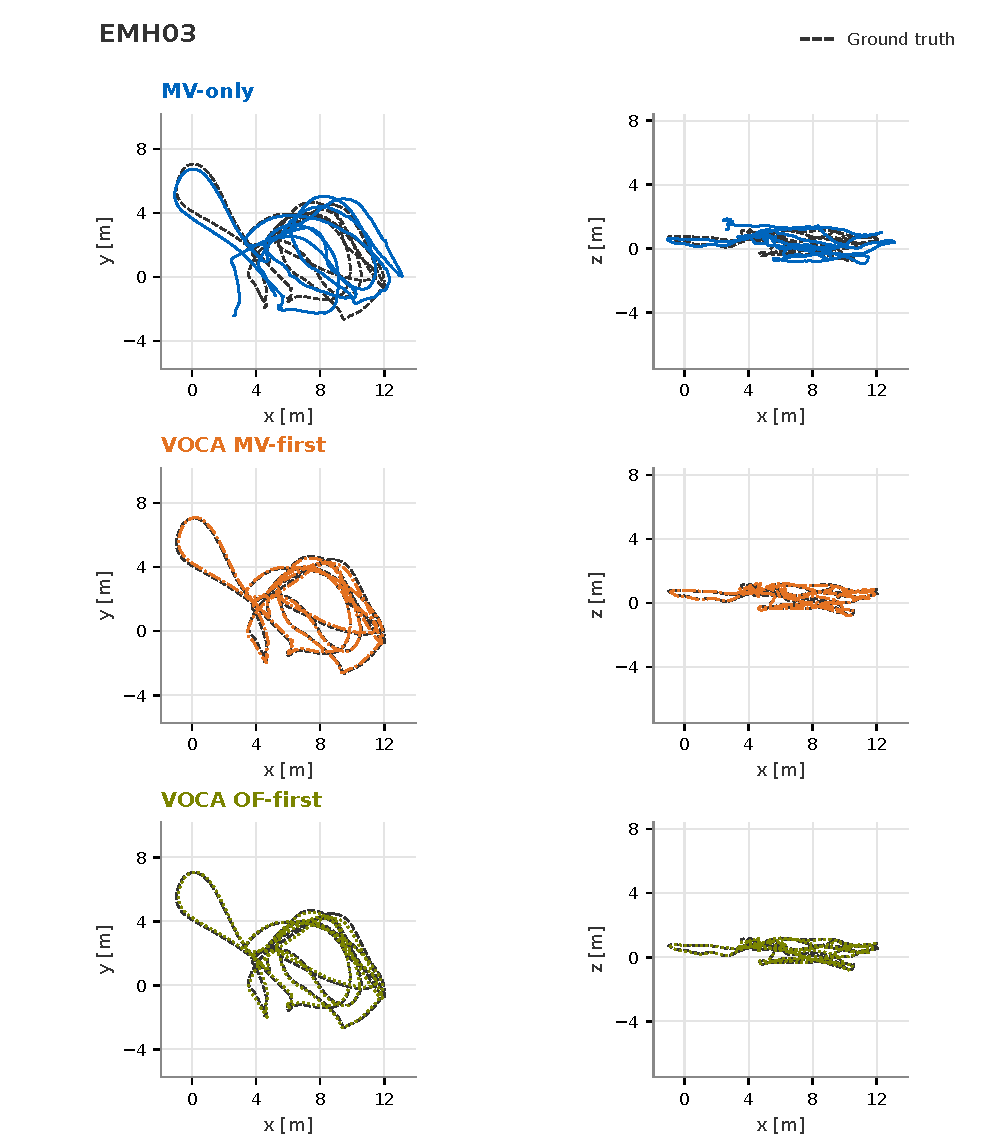
\includegraphics[width=\textwidth]{figures/evaluation/trajectory-emh03-separated.pdf}
  \caption[EMH03 trajectory comparison]{Full-sequence EMH03 trajectories. Top to bottom: MV-only,
  VOCA MV-first, and VOCA OF-first, each with ground truth. Left: $xy$;
  right: $xz$. Alignment and plotting conventions follow
  \autoref{fig:trajectory-emh01-separated}.}
  \label{fig:trajectory-emh03-separated}
\end{figure}

\begin{figure}[p]
  \centering
  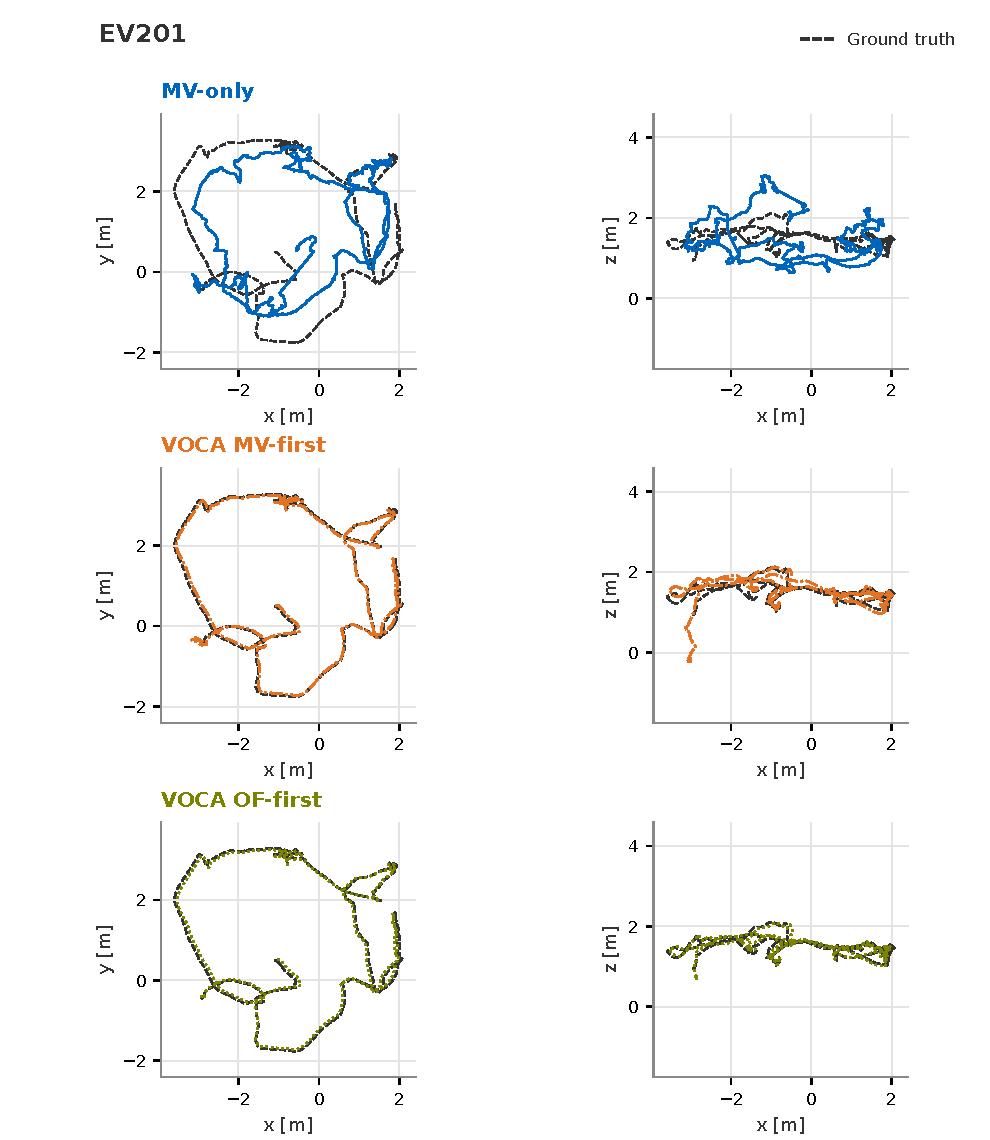
\includegraphics[width=\textwidth]{figures/evaluation/trajectory-ev201-separated.pdf}
  \caption[EV201 trajectory comparison]{Full-sequence EV201 trajectories. Top to bottom: MV-only,
  VOCA MV-first, and VOCA OF-first, each with ground truth. Left: $xy$;
  right: $xz$. Alignment and plotting conventions follow
  \autoref{fig:trajectory-emh01-separated}.}
  \label{fig:trajectory-ev201-separated}
\end{figure}

\clearpage

\section{Results by Sequence Difficulty}

For PVO, the easy sequences have a mean ATE of
\SI{0.500}{\metre} and a median of \SI{0.420}{\metre}. The corresponding values
are \SI{1.228}{\metre} and \SI{1.082}{\metre} for the medium sequences, and
\SI{6.968}{\metre} and \SI{5.609}{\metre} for the difficult sequences. Mean
RTE-6 rises from \SI{0.0306}{\metre} on easy sequences to
\SI{0.0971}{\metre} on medium and \SI{0.7035}{\metre} on difficult sequences.

These labels are descriptive groups, not uniformly spaced levels of numeric
difficulty. EV201, for example, is labelled easy but its codec-only ATE is higher
than that of the other three easy sequences. Conversely, local RTE-6 remains
relatively small on some trajectories whose global ATE is poor.

\begin{table}[htbp]
  \centering
  \caption[Trajectory and track statistics by sequence difficulty]{Trajectory and track statistics of PVO grouped by
  the EuRoC difficulty labels. Observations/frame counts confirmed
  anchor-camera observations pooled over input frames, not new identities or
  connected backend landmarks. Lifetimes are pooled over tracks;
  trajectory means and medians weight sequences equally.}
  \label{tab:difficulty-track-summary}
  \resizebox{\textwidth}{!}{%
  \begin{tabular}{@{}lrrrrrrrr@{}}
    \toprule
    & \multicolumn{2}{c}{ATE [m]} & \multicolumn{2}{c}{RTE-6 [m]}
    & & \multicolumn{3}{c}{Track lifetime} \\
    \cmidrule(lr){2-3}\cmidrule(lr){4-5}\cmidrule(l){7-9}
    Difficulty & Mean & Median & Mean & Median & Obs./frame
      & Mean [frames] & $\geq5$ [\%] & Maximum \\
    \midrule
    Easy      & 0.500 & 0.420 & 0.0306 & 0.0156 & 998.21 & 3.521 & 11.04 & 204 \\
    Medium    & 1.228 & 1.082 & 0.0971 & 0.0476 & 475.11 & 3.403 & 8.11 & 77 \\
    Difficult & 6.968 & 5.609 & 0.7035 & 0.3256 & 370.99 & 3.415 & 7.67 & 82 \\
    \bottomrule
  \end{tabular}}
\end{table}

\begin{figure}[htbp]
  \centering
  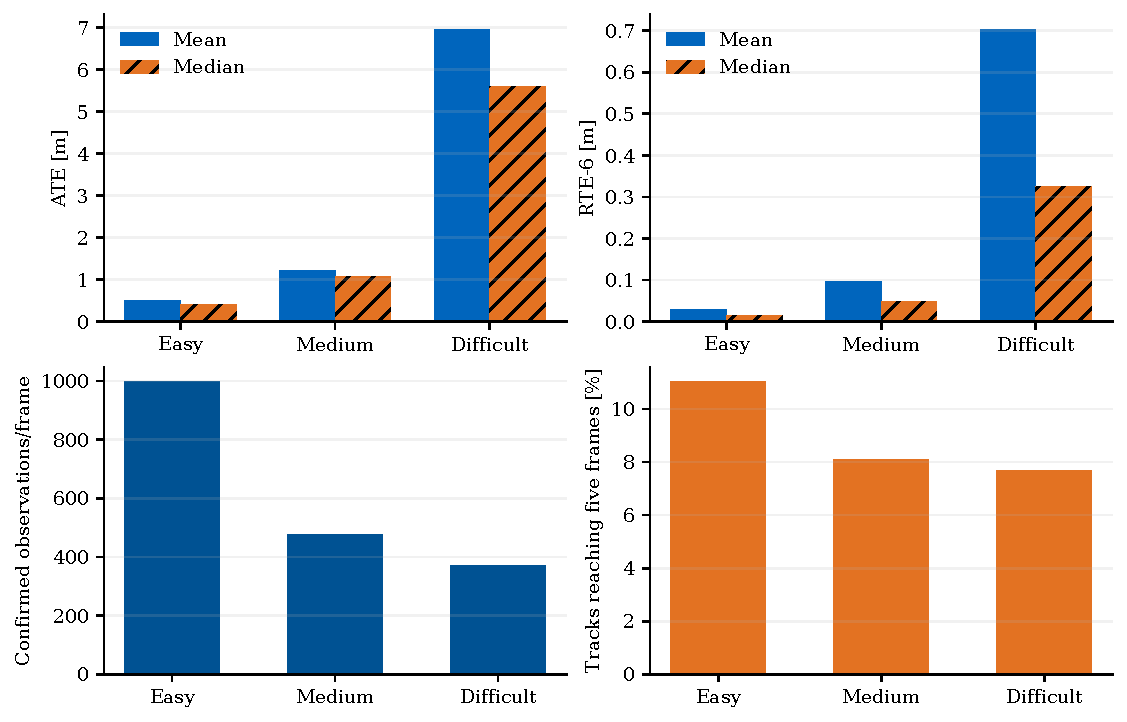
\includegraphics[width=\textwidth]{figures/evaluation/difficulty-summary}
  \caption[Trajectory errors and track support by sequence difficulty]{PVO trajectory errors and track support separated by
  EuRoC difficulty. Confirmed observation density decreases across the groups,
  while all three remain dominated by short tracks. The lifetime panel reports
  the proportion reaching at least five frames.}
  \label{fig:difficulty-summary}
\end{figure}

\clearpage

\section{Component Ablation}

\autoref{tab:component-ablation-ate} and
\autoref{tab:component-ablation-rte} give the full-sequence component results at
the original operating point and the selected PVO result. Bold marks the lowest
codec-only value in each row. ``Joint frontend'' uses the complete method at the
original settings; PVO uses the same components with selected reciprocal gates,
suppression distance, observation standard deviation, and Huber threshold.
PVO is included for comparison but is not another cell of the controlled
component ablation.

\begin{table}[htbp]
  \centering
  \caption[Component ablation: absolute trajectory error]{Full-sequence ATE for the codec-only component ablation, in metres.}
  \label{tab:component-ablation-ate}
  \resizebox{\textwidth}{!}{%
  \begin{tabular}{@{}lrrrrr@{}}
    \toprule
    Sequence & TEASER++ only & F-B agreement & Suppression & Joint frontend & PVO \\
    \midrule
    EMH01 & \textbf{0.129} & 0.488 & 0.143 & 0.232 & 0.246 \\
    EMH02 & 0.310 & 0.352 & 0.296 & \textbf{0.203} & 0.594 \\
    EMH03 & 3.261 & 1.559 & 1.508 & 1.569 & \textbf{1.082} \\
    EMH04 & \textbf{3.527} & 6.045 & 4.856 & 5.672 & 4.722 \\
    EMH05 & 5.629 & 5.401 & 4.706 & 5.318 & \textbf{4.089} \\
    EV101 & 0.381 & 0.340 & 0.434 & \textbf{0.223} & 0.226 \\
    EV102 & 0.596 & \textbf{0.501} & 0.594 & 0.622 & 0.514 \\
    EV103 & 2.536 & 2.196 & \textbf{2.019} & 3.406 & 12.565 \\
    EV201 & 1.673 & \textbf{0.727} & 1.968 & 0.899 & 0.935 \\
    EV202 & 2.495 & 2.392 & \textbf{2.040} & 2.671 & 2.087 \\
    EV203 & \textbf{4.842} & 5.817 & 6.479 & 7.635 & 6.497 \\
    \midrule
    Macro mean & 2.307 & 2.347 & \textbf{2.277} & 2.586 & 3.051 \\
    Median & 2.495 & 1.559 & 1.968 & 1.569 & \textbf{1.082} \\
    \bottomrule
  \end{tabular}}
\end{table}

\begin{table}[htbp]
  \centering
  \caption[Component ablation: six-frame relative translation error]{Full-sequence RTE-6 for the codec-only component ablation, in
  metres.}
  \label{tab:component-ablation-rte}
  \resizebox{\textwidth}{!}{%
  \begin{tabular}{@{}lrrrrr@{}}
    \toprule
    Sequence & TEASER++ only & F-B agreement & Suppression & Joint frontend & PVO \\
    \midrule
    EMH01 & \textbf{0.0091} & 0.0118 & 0.0092 & 0.0115 & 0.0092 \\
    EMH02 & \textbf{0.0112} & 0.0155 & 0.0112 & 0.0159 & 0.0123 \\
    EMH03 & 0.0848 & 0.1025 & 0.0477 & 0.0978 & \textbf{0.0476} \\
    EMH04 & 0.1779 & 0.1767 & 0.1476 & 0.1488 & \textbf{0.1344} \\
    EMH05 & 0.1414 & 0.2290 & 0.1226 & 0.1365 & \textbf{0.1195} \\
    EV101 & 0.0363 & 0.0252 & 0.0343 & 0.0190 & \textbf{0.0189} \\
    EV102 & 0.0368 & 0.0480 & 0.0365 & 0.0494 & \textbf{0.0359} \\
    EV103 & 0.3264 & \textbf{0.2262} & 0.2839 & 0.2585 & 2.0434 \\
    EV201 & 0.2674 & 0.1134 & 0.4599 & 0.1005 & \textbf{0.0818} \\
    EV202 & 0.2328 & 0.2735 & 0.2102 & 0.2564 & \textbf{0.2078} \\
    EV203 & 0.5989 & 0.4523 & 0.7135 & \textbf{0.4365} & 0.5169 \\
    \midrule
    Macro mean & 0.1748 & 0.1522 & 0.1888 & \textbf{0.1392} & 0.2934 \\
    Median & 0.1414 & 0.1134 & 0.1226 & 0.1005 & \textbf{0.0818} \\
    \bottomrule
  \end{tabular}}
\end{table}

\clearpage

PVO has the lowest median ATE and RTE-6 and the lowest RTE-6 on seven sequences.
Suppression at the original operating point retains the lowest macro mean ATE,
while the joint frontend at that point retains the lowest macro mean RTE-6. The
PVO macro means are dominated by the EV103 failure. Relative to TEASER++ only,
PVO lowers ATE on six sequences and RTE-6 on eight. The sequence rows make the
non-monotonic effect explicit: the selected parameters improve typical local
drift but do not eliminate large failures.

\section{Observation-Model Ablation}

The paired comparison in \autoref{tab:residual-ablation} uses the complete
selected PVO frontend and changes only the backend observation factor. The
rigid-flow residual has lower ATE on eight of eleven sequences and lower RTE-6
on seven. It also lowers both medians. The macro means favour absolute
reprojection because the rigid-flow run fails strongly on EV103, and absolute
reprojection is also better on EV203. The displacement formulation therefore
improves the typical sequence in this experiment but does not remove the
method's sequence-level failure modes.

\begin{table}[p]
  \centering
  \caption[Ablation of the observation model]{Full-sequence ablation of the observation model at the selected PVO
  operating point. All encoded inputs, frontend decisions, robust associations,
  loss parameters, and window settings are shared. Lower is better; bold marks
  the lower value within each metric.}
  \label{tab:residual-ablation}
  \begin{tabular}{@{}lrrrr@{}}
    \toprule
    & \multicolumn{2}{c}{ATE [m]} & \multicolumn{2}{c}{RTE-6 [m]} \\
    \cmidrule(lr){2-3}\cmidrule(l){4-5}
    Sequence & Absolute & Rigid flow & Absolute & Rigid flow \\
    \midrule
    EMH01 & 0.253 & \textbf{0.246} & \textbf{0.0089} & 0.0092 \\
    EMH02 & \textbf{0.482} & 0.594 & 0.0207 & \textbf{0.0123} \\
    EMH03 & 1.215 & \textbf{1.082} & 0.0488 & \textbf{0.0476} \\
    EMH04 & 4.960 & \textbf{4.722} & \textbf{0.1294} & 0.1344 \\
    EMH05 & 4.266 & \textbf{4.089} & 0.1279 & \textbf{0.1195} \\
    EV101 & 0.263 & \textbf{0.226} & 0.0219 & \textbf{0.0189} \\
    EV102 & 0.531 & \textbf{0.514} & 0.0393 & \textbf{0.0359} \\
    EV103 & \textbf{2.538} & 12.565 & \textbf{0.2910} & 2.0434 \\
    EV201 & 1.152 & \textbf{0.935} & 0.0824 & \textbf{0.0818} \\
    EV202 & 2.281 & \textbf{2.087} & 0.2621 & \textbf{0.2078} \\
    EV203 & \textbf{4.565} & 6.497 & \textbf{0.4264} & 0.5169 \\
    \midrule
    Macro mean & \textbf{2.046} & 3.051 & \textbf{0.1326} & 0.2934 \\
    Median & 1.215 & \textbf{1.082} & 0.0824 & \textbf{0.0818} \\
    \bottomrule
  \end{tabular}
\end{table}

\section{Track Length and Geometric Support}

Across all eleven sequences, PVO produces 5,230,916 confirmed
tracks. Their mean length is 3.48 frames, the median is 3, the 90th percentile is
4, the 95th percentile is 5, and the longest track spans 204 frames. Only
29.85\% survive for at least four frames, 9.92\% for at least five, 0.25\% for at
least ten, and 0.05\% for at least twenty. The method therefore creates
persistent identities, but the typical constraint has little multiview support.

No quantitative track-length comparison with the VOCA MV-first and OF-first
references is reported. The necessary lifetime instrumentation was evaluated in
a separate diagnostic build that did not reproduce the frozen reference
trajectories: its ATE on the first easy Machine Hall sequence differed from both
reference values. Retaining those track statistics would therefore mix
different operating points. The trajectory comparison in
\autoref{tab:euroc-ate} and \autoref{tab:euroc-rte6} remains valid because it
uses the archived frozen reference results directly.

The stereo-query yield also varies substantially by sequence. In PVO it is
13.48\% on EMH01, 13.56\% on EMH02, and 19.88\% on EV101, but falls to 1.99\%,
1.14\%, and 0.71\% on EV201 to EV203. Among observations with depth at
consecutive endpoints, the mean absolute depth change ranges from
\SI{0.0262}{\metre} to \SI{0.0424}{\metre}. This conditional statistic does not
measure the larger population for which one or both depths are absent.

\autoref{fig:stereo-depth-support} retains the individual sequence measurements
alongside the signed RTE-6 difference, PVO minus VOCA MV-first. The plot describes
which support measurements accompany each complete trajectory; it does not
locate a failure or identify its cause. In particular, similar full-sequence
track lifetimes can conceal a brief interruption or an extended period of
incorrect motion. \autoref{sec:failure-episodes} examines those events in their
temporal and visual context.

\begin{figure}[htbp]
  \centering
  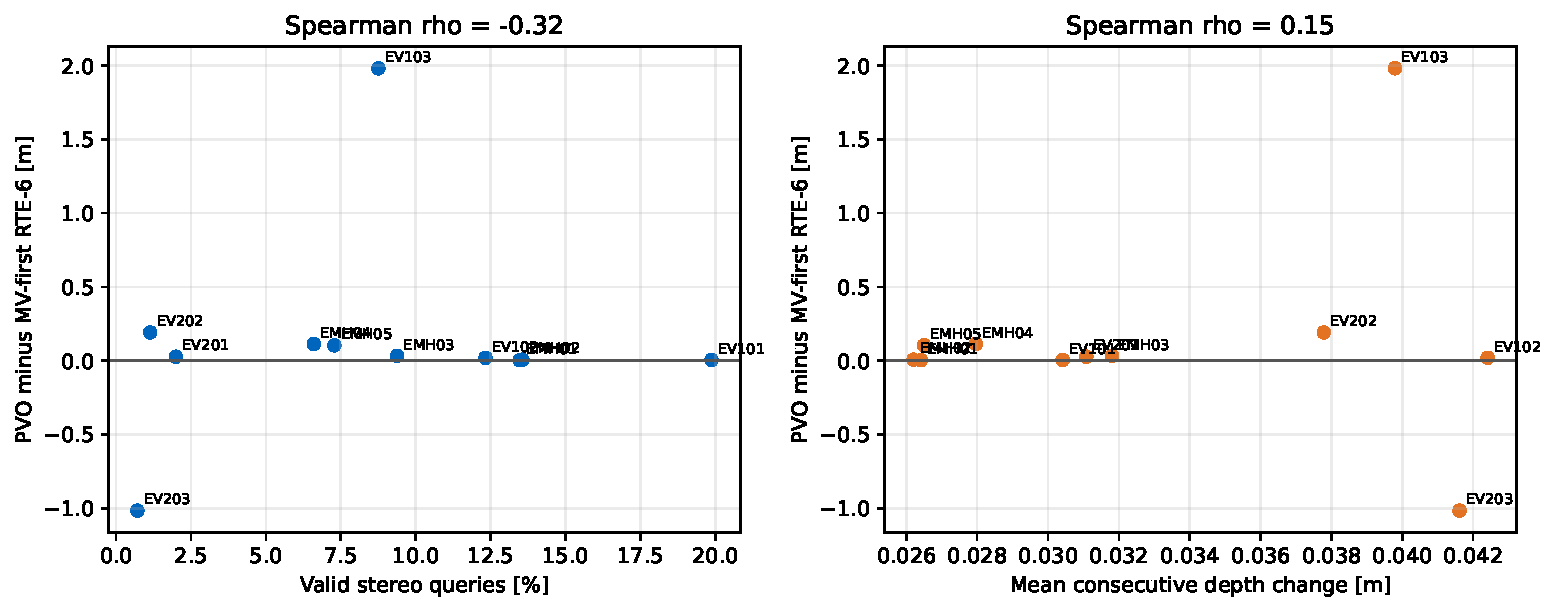
\includegraphics[width=\textwidth]{figures/evaluation/stereo-and-depth-support}
  \caption[Stereo support and relative translation error]{Valid-stereo rate (left) and mean absolute consecutive depth change
  (right) against the signed RTE-6 difference, PVO minus VOCA MV-first.
  Positive vertical values indicate greater PVO error. Labels identify the
  eleven sequence aggregates.}
  \label{fig:stereo-depth-support}
\end{figure}

\section{Coincidence with Conventional Image Structure}

The error-surface analysis in \autoref{eq:mv-error-hessian} provides the reason
for measuring this coincidence. Corner-like structure gives a block matching
cost curvature in two displacement directions, whereas an edge or weakly
textured support leaves at least one direction ambiguous. The following test
therefore measures whether filtering concentrates motion-vector support near
image structure that can condition translational matching; it does not label a
motion vector as geometrically correct.

Decoded images are used only in this offline diagnostic. The estimator itself
does not receive the Shi-Tomasi responses reported in
\autoref{tab:structure-support-all}. A motion-vector observation is counted as
structurally coincident when its exact prediction-block rectangle contains at
least one Shi-Tomasi corner. The rows give an ordered processing summary: raw anchor-camera
temporal vectors, vectors with valid stereo depth at both temporal endpoints,
reciprocal forward-backward candidates, TEASER++ survivors, and candidates
retained after age-prioritized suppression. The retained row also includes new
best-direction births awaiting reciprocal confirmation, so it branches from the
strict reciprocal path rather than forming its final subset.

\begin{table}[htbp]
  \centering
  \caption[Coincidence of codec supports and image corners]{Pooled full-sequence Shi-Tomasi coincidence across all eleven EuRoC
  sequences. Region support is the fraction of codec regions containing a
  corner; feature coverage is the fraction of detected corners lying in the
  union of those regions.}
  \label{tab:structure-support-all}
  \begin{tabular}{@{}lrrr@{}}
    \toprule
    Stage & Regions & Regions with corner & Corner coverage \\
    \midrule
    Raw temporal MVs & 84,675,992 & 30.59\% & 98.58\% \\
    Valid stereo depth & 41,353,155 & 37.45\% & 59.88\% \\
    Forward-backward candidates & 13,899,680 & 34.38\% & 32.48\% \\
    TEASER++ survivors & 6,856,688 & 39.57\% & 18.70\% \\
    Suppression-retained candidates & 23,057,616 & 44.54\% & 43.03\% \\
    \bottomrule
  \end{tabular}
\end{table}

Requiring stereo depth raises the region-level corner ratio from 30.59\% to
37.45\%. Contrary to a monotonic-enrichment hypothesis, reciprocal agreement
then lowers it to 34.38\%. TEASER++ raises it to 39.57\%, while the branched
suppression-retained pool reaches 44.54\%. The first four candidate counts fall
at every stage, so TEASER++ is both selective and more concentrated near
Shi-Tomasi structure than its reciprocal input. The feature-coverage column is
reported separately because the dense raw block union covers nearly every
corner even when individual regions are poorly localized.

\begin{figure}[htbp]
  \centering
  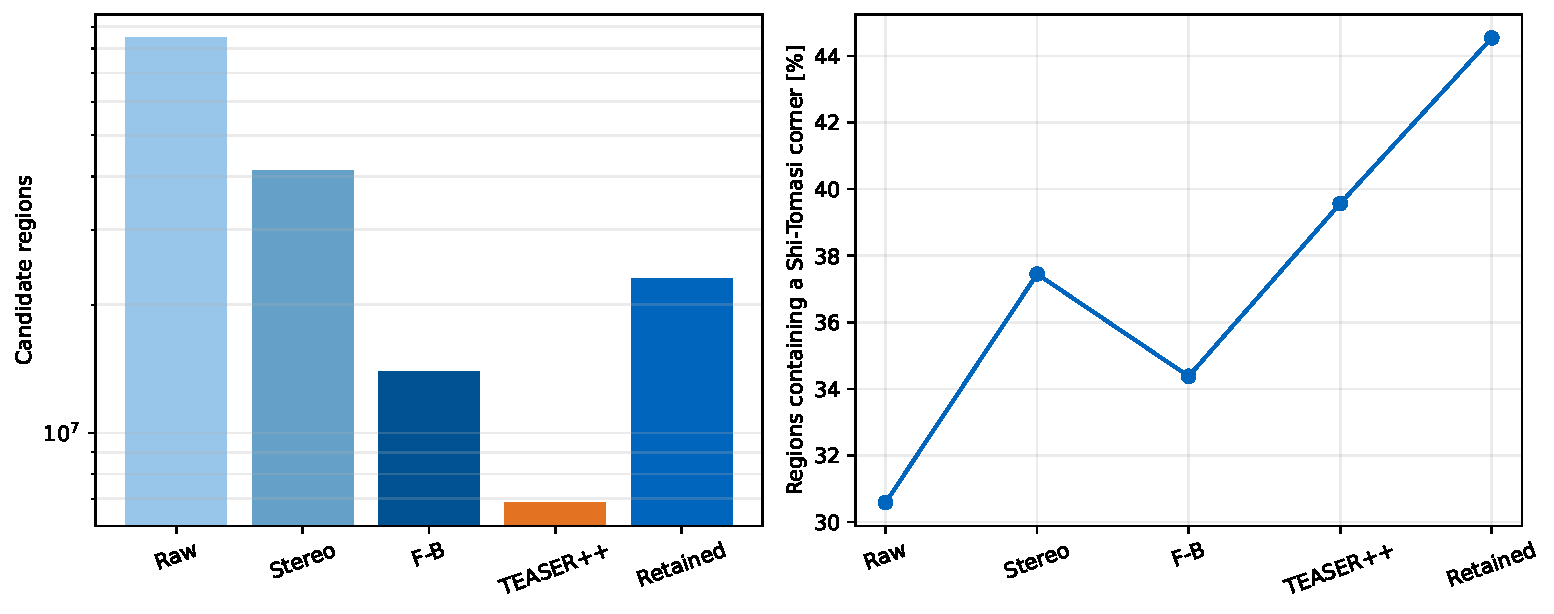
\includegraphics[width=\textwidth]{figures/evaluation/feature-support-funnel}
  \caption[Candidate count and structural support through filtering]{Candidate count and structural coincidence through the codec-only
  selection stages, pooled over all eleven sequences.}
  \label{fig:feature-support-funnel}
\end{figure}

Stricter Shi-Tomasi quality levels test whether the coincidence is limited to
weak corner responses. The same final codec supports are held fixed while only
the offline diagnostic threshold changes.

\begin{table}[htbp]
  \centering
  \caption[Corner coincidence at different detector thresholds]{Pooled coincidence of final codec supports with Shi-Tomasi corners
  at increasingly selective quality levels.}
  \label{tab:detector-threshold-support}
  \begin{tabular}{@{}lrrr@{}}
    \toprule
    Quality level & Corners & Regions with corner & Corner coverage \\
    \midrule
    0.01 & 18,921,761 & 44.54\% & 43.03\% \\
    0.05 & 8,365,939 & 25.51\% & 48.39\% \\
    0.10 & 5,076,456 & 17.64\% & 51.75\% \\
    \bottomrule
  \end{tabular}
\end{table}

At the default quality level, 44.54\% of retained regions contain a corner and
their union covers 43.03\% of the detected corners. As the diagnostic retains
only stronger corners, region coincidence falls because fewer responses exist,
but coverage of those responses rises to 51.75\%. This does not imply that a
retained codec region is a uniquely localized feature or that the estimator
observes the corner response.

\begin{figure}[htbp]
  \centering
  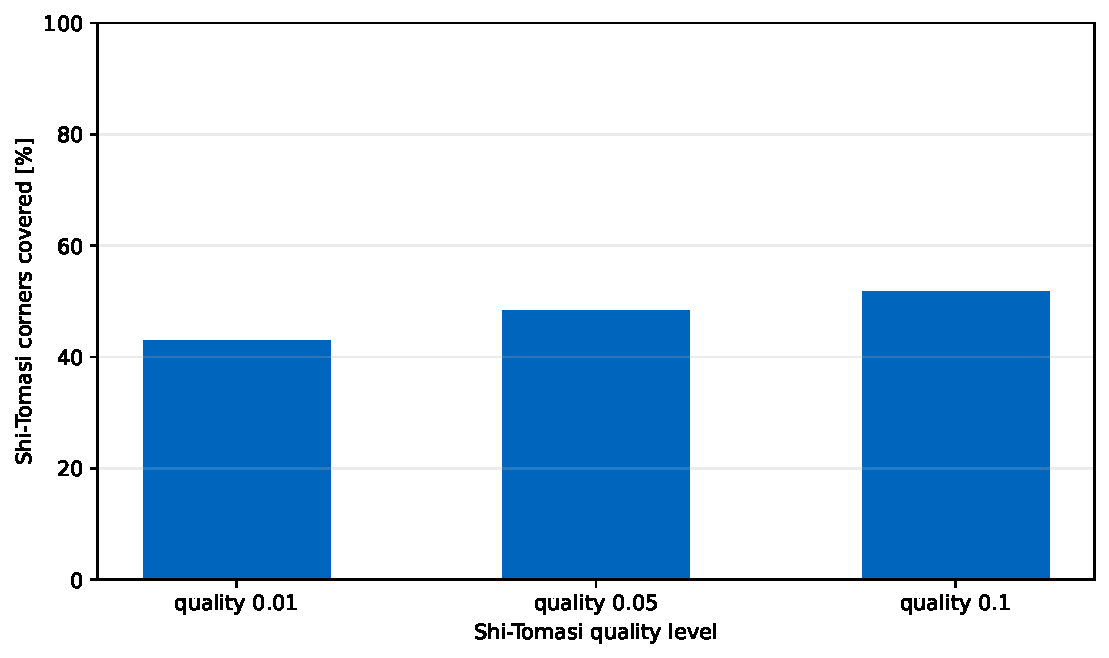
\includegraphics[width=0.8\textwidth]{figures/evaluation/shi-tomasi-threshold-support}
  \caption[Corner coverage at different detector thresholds]{Pooled Shi-Tomasi corner coverage by the fixed final codec supports
  at three detector quality levels.}
  \label{fig:shi-tomasi-threshold-support}
\end{figure}

\section{Reference Configurations}

The MV-first and OF-first VOCA configurations have access to image intensities
that are deliberately unavailable to the proposed estimator. They therefore
serve as higher-information operating points rather than objectives that the
PVO is expected to surpass. Their median ATE values are
\SI{0.200}{\metre} and \SI{0.118}{\metre}, respectively, compared with
\SI{1.082}{\metre} for PVO. Median RTE-6 is
\SI{0.0163}{\metre} for VOCA MV-first, \SI{0.0155}{\metre} for VOCA OF-first,
and \SI{0.0818}{\metre} for PVO.

The macro mean alone obscures reference failures: VOCA MV-first reaches
\SI{9.532}{\metre} ATE and \SI{1.534}{\metre} RTE-6 on EV203. The per-sequence
tables and empirical distributions are therefore retained rather than reducing
the benchmark to a single ranking. The central result is that codec side
information alone supports non-stationary estimates on a substantial part of the
benchmark, while a large and sequence-dependent accuracy gap remains.

% !TeX root = ../main.tex

\section{Failure Episodes}\label{sec:failure-episodes}

The full-sequence errors can arise through markedly different events. The
following cases follow the observations and estimated motion before, during,
and after an error. They use the selected PVO runs, with the paired absolute
residual and frozen VOCA OF-first results where indicated. The intervals were
selected by inspecting the complete saved trajectories; they are illustrative
episodes, not a partition of the benchmark or a model that predicts failure.
Times in the figures are relative to the first ground-truth-associated pose of
the sequence. Exact intervals and sources are retained with the analysis assets.

\subsection{Sustained Drift in a Dark, Sparsely Detailed View}

On EMH04, the view changes from machinery and pipework to a broad cabin roof
and the dark hall behind it. \autoref{fig:failure-emh04} follows this transition.
During a \SI{7.8}{\second} interval of sustained error, the images contain an
average of 124 Shi-Tomasi corners, compared with 751 in a later interval with
more visible machinery. RTE-6 falls from \SI{0.3584}{\metre} during the
degraded interval to \SI{0.0209}{\metre} in the later interval, even though mean
ground-truth path speed increases from \SI{1.19}{\metre\per\second} to
\SI{1.37}{\metre\per\second}. Faster translation therefore does not account
for the difference between these two views.

Codec candidates remain abundant. The degraded interval contains approximately
2229 temporal candidates per frame with valid stereo at both endpoints, and
217 current IDs per frame are connected to existing backend landmarks. These
counts do not collapse to zero. The estimated motion nevertheless becomes
incorrect in both magnitude and direction, and the first-pose-aligned
orientation error grows to approximately \SI{67}{\degree}. Once the view
improves, local translation error becomes small again, but much of the
orientation error remains. Local recovery therefore does not imply recovery
of the accumulated trajectory.

\begin{figure}[p]
  \centering
  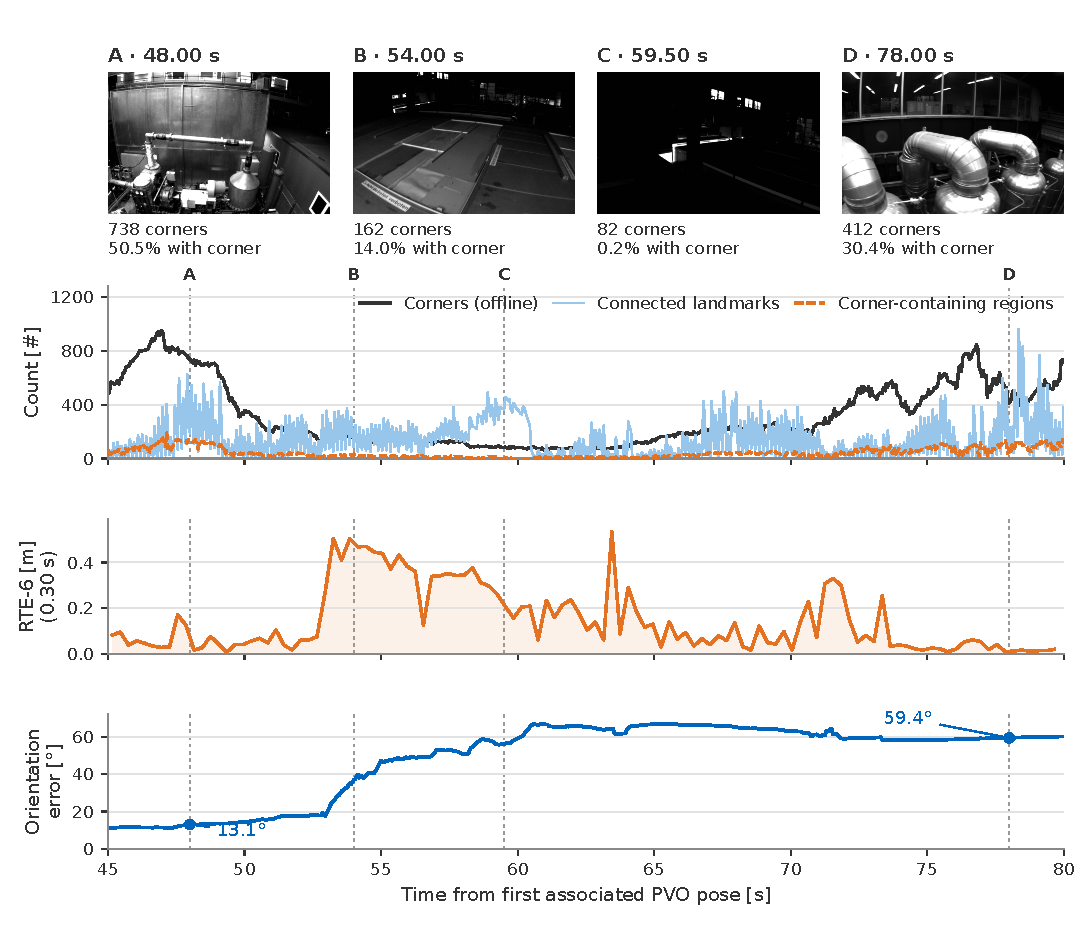
\includegraphics[width=\textwidth]{figures/evaluation/emh04-dark-scene-progression}
  \caption[Sustained drift on EMH04]{EMH04 before, during, and after sustained drift. Raw anchor-camera
  images are shown only for diagnosis. The synchronized traces distinguish
  changing image structure, local translation error, and persistent orientation
  error. Corner-containing regions are TEASER-stage MV destination blocks
  containing at least one offline Shi-Tomasi corner; the percentages divide
  their count by all logged TEASER-stage regions in each sampled frame.
  Connected IDs instead count observations linked to existing backend landmarks.
  Orientation error is aligned at the first pose, not over the full trajectory.}
  \label{fig:failure-emh04}
\end{figure}

The images and support measurements are consistent with less informative
codec predictions over broad surfaces and dark regions. The connection to
block-matching ambiguity follows the error-surface argument in
\autoref{eq:mv-error-hessian}~\cite{zhang2010subpixel,shi1994good}.
However, the recorded counts do not measure disparity accuracy or the spatial
rank of the retained point set. They cannot distinguish incorrect stereo
depth, temporal displacement bias, and unfavorable point geometry as the main
source of this episode. The fact that the paired absolute-residual run also
degrades in this interval provides an additional limit on its interpretation.

\subsection{A Brief Loss of Connections During Rapid Motion}

EMH03 contains a shorter event in which a six-frame interval reaches
\SI{0.4423}{\metre} RTE-6. It has an average of only 12.6 current IDs connected
to existing landmarks. A separate rapid-motion interval in the same sequence
has slightly greater translation and angular speed, yet its RTE-6 is only
\SI{0.0265}{\metre}. That interval retains 186.4 connected IDs on average.
The two image intervals contain similar numbers of detected corners, 656 and
670 per frame, respectively.

\begin{figure}[p]
  \centering
  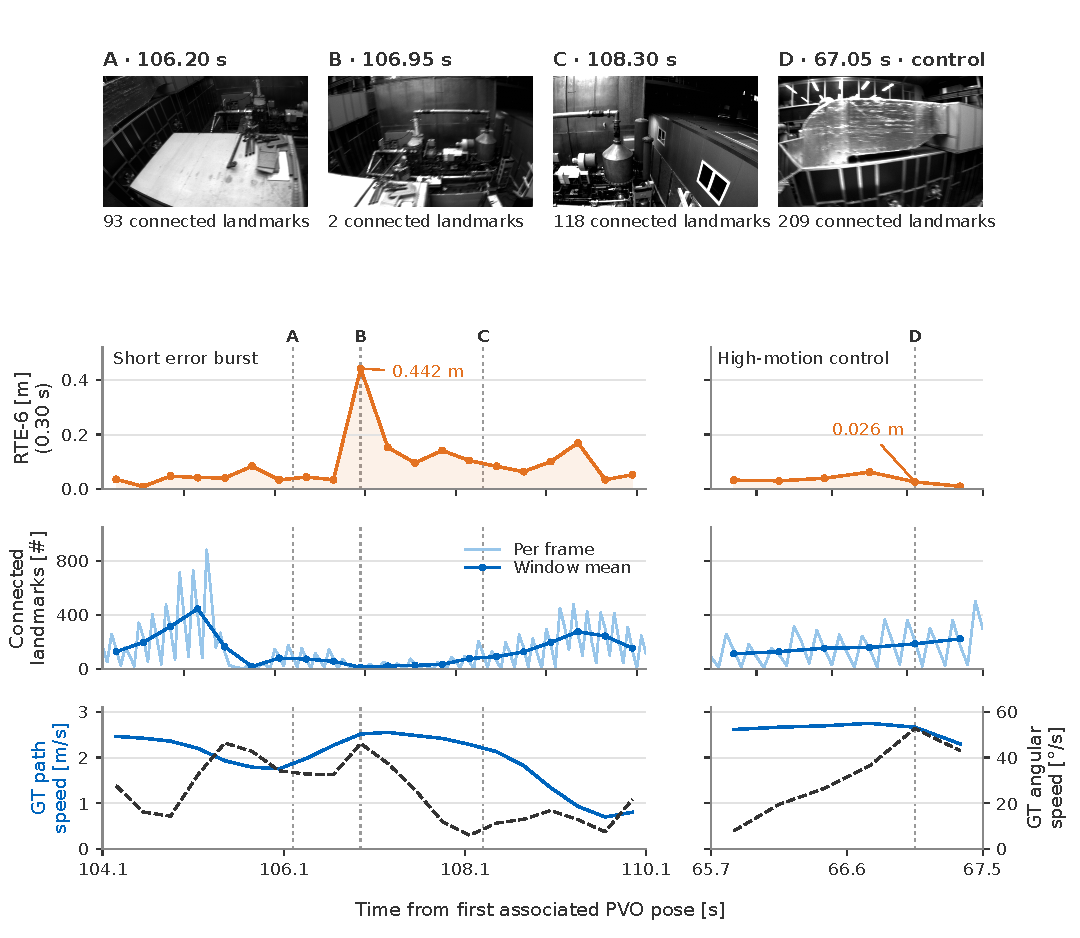
\includegraphics[width=\textwidth]{figures/evaluation/emh03-short-burst-and-motion-control}
  \caption[EMH03 error burst and rapid-motion comparison]{A short EMH03 error burst and a rapid-motion comparison interval.
  Connected IDs are current observations linked to existing backend landmarks.
  Similar image corner counts do not imply similar surviving temporal support;
  the faster comparison interval retains substantially more connections.}
  \label{fig:failure-emh03}
\end{figure}

This comparison separates the availability of visible structure from its
conversion into persistent observations. The failed interval is not simply
the faster or less corner-rich of the two. Its small connected set coincides
with a large local error, although the archived counters do not identify which
individual candidate losses produced that set. The absolute-residual run has
almost the same error in the burst, \SI{0.4397}{\metre}, which again indicates
that replacing rigid flow alone does not remove the event.

\subsection{Missing Temporal Observations, a Pose Jump, and a Stall}

EV103 illustrates a discontinuity rather than gradual drift. The view
approaches a bright window beside a broad dark partition. Visible corners and
emitted track IDs decrease. Inspection of the encoded streams also identifies
an I-frame in each direction at the endpoints of one temporal transition,
leaving no ordinary temporal MVs for that connection. Three frames later,
the estimated pose jumps by \SI{37.716}{\metre} and rotates by
\SI{174.42}{\degree} in one frame. Ground truth changes by only
\SI{0.050}{\metre} and \SI{0.77}{\degree}. At the jump, only two current IDs
are connected to existing landmarks; the optimizer records eight iterations,
six of them rejected.

\begin{figure}[p]
  \centering
  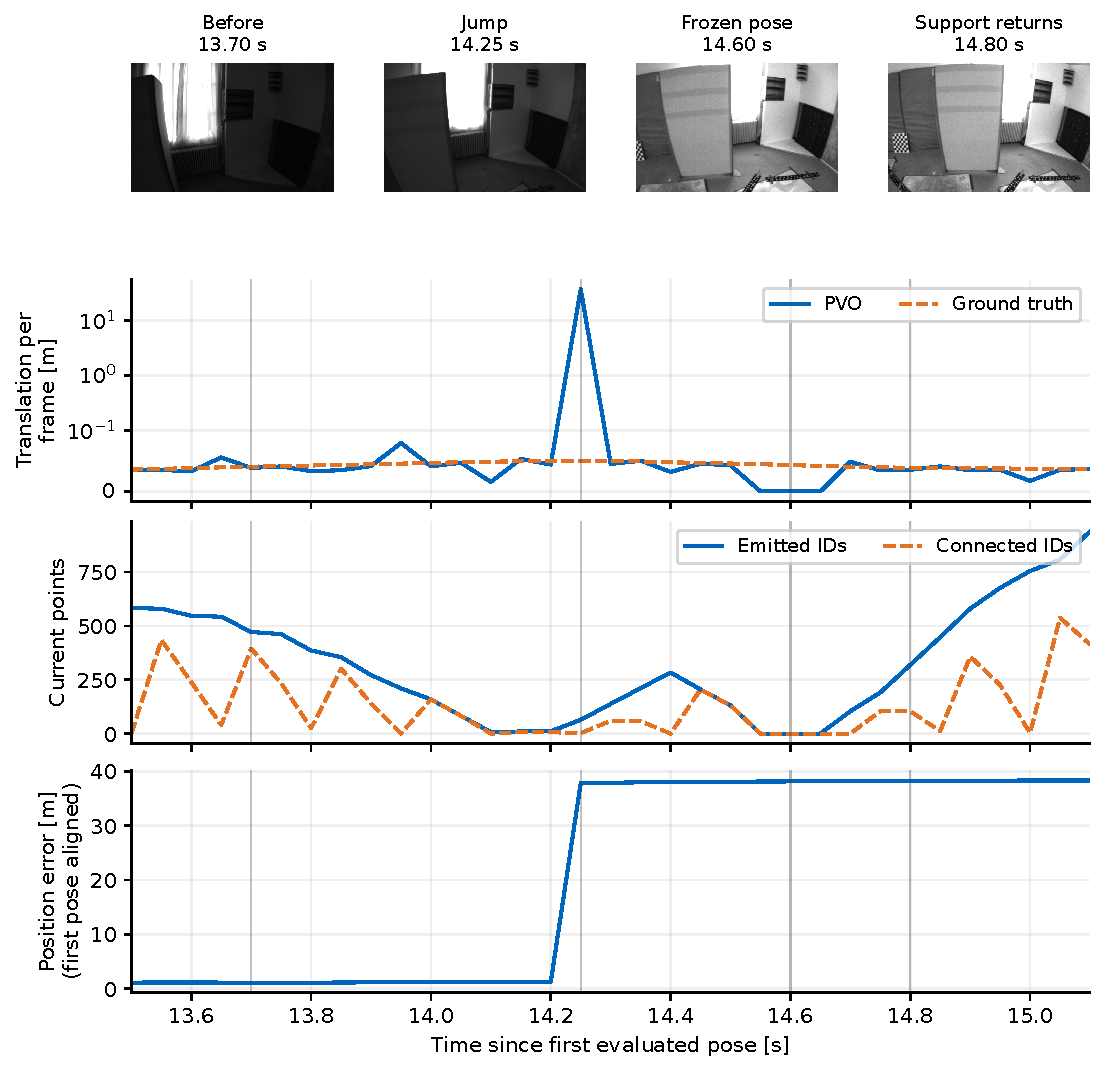
\includegraphics[width=\textwidth]{figures/evaluation/failure-ev103-jump}
  \caption[Catastrophic pose update on EV103]{EV103 around a catastrophic pose update. Per-frame translation uses
  a symmetric logarithmic axis so that ordinary motion, the large jump, and
  zero-motion outputs remain visible. The lower panels show the temporary loss
  of frontend support and the persistent position error after support returns.
  The sampled images are offline diagnostics.}
  \label{fig:failure-ev103}
\end{figure}

A subsequent transition again lacks temporal MVs in both directions. The
frontend then emits zero points for three consecutive frames and the pose
remains exactly unchanged, although ground truth moves approximately
\SI{0.04}{\metre} per frame. Image corners have already returned to at least
350 per frame. Raw MV candidates return after the missing transition, but no
candidate survives the logged stage requiring filtering and valid stereo at
both endpoints for the next two frames. These records locate the loss within
the processing chain; they do not isolate the median filter from stereo lookup
as its cause. Connections subsequently return, while the accumulated position
error remains approximately \SI{38}{\metre}.

The I-frames explain the observed absence of temporal vectors at particular
transitions, not the complete sequence of errors. The catastrophic update
itself occurs on a P-frame, and the shortage of usable observations extends
beyond the I-frame. The containing six-frame window contributes 98.6\% of
the full sequence's sum of squared six-frame translation errors. Its RTE-6 is
\SI{37.8510}{\metre}, compared with \SI{0.4066}{\metre} in the paired
absolute-residual run. This episode exposes a strong difference in how the
backends respond to the available observations; it does not show that every
large PVO error has the same origin.

\subsection{Low-Motion Errors and a Textured Counterexample}

EV202 contains consecutive estimated translations of \SI{1.117}{\metre} and
\SI{0.895}{\metre} while ground truth moves only \SI{0.013}{\metre} in each
frame. The images change little and show fabric-covered blocks, a plain wall,
and a small cart. Only three and two IDs, respectively, connect to existing
landmarks. At the first jump, 2919 raw MV regions and 541 stereo-valid temporal
candidates are still available, but only 25 reciprocal candidates and four
candidates passing the fitted rigid-model gate remain. This is another case
in which many initial observations do not translate into substantial temporal
support.

A later EV202 event provides a counterexample to using image corner count as a
sufficient indicator. A close, textured fabric surface dominates the view and
1640 corners are detected, yet the estimated translation is
\SI{0.752}{\metre} against a ground-truth step of \SI{0.015}{\metre}. Only six
IDs connect to existing landmarks. Conversely, a separate six-frame interval
with an average of 7.4 connected IDs has RTE-6 of only \SI{0.0376}{\metre}.
Neither high corner count nor low connection count alone determines the
outcome. Supplementary images and per-frame values are given in
\autoref{appendix:failure-episode-details}.

\subsection{What the Paired Residual Comparison Establishes}

\autoref{tab:episode-residual-comparison} compares identical timestamp
intervals from PVO, its absolute-residual ablation, and the frozen VOCA
OF-first reference. The two PVO runs share encoded inputs and frontend settings,
including the robust association procedure. EMH03's brief burst and EMH04's sustained error
remain under absolute reprojection. EV103's catastrophic amplification is much
smaller with absolute reprojection, as is EV202's textured-view error.
However, the EV202 jump at \SI{38.30}{\second} becomes larger. The observation
model thus changes the response to particular
correspondence sets without providing a universal safeguard. The low OF-first
errors on the same intervals show that the camera sequences still contain
information from which the richer reference can recover motion.

\begin{table}[htbp]
  \centering
  \caption[Observation-model comparison over failure episodes]{RTE-6 in metres; lower is better. Entries report
  RMSE over the listed non-overlapping windows. Absolute changes PVO's
  observation model; OF-first is the frozen pixel-refined reference. The
  EV202 middle jump is at \SI{38.30}{\second}, distinct from the later
  textured-view event.}
  \label{tab:episode-residual-comparison}
  \begin{tabular}{@{}lrrrr@{}}
\toprule
Episode & Windows & PVO [m] & Absolute [m] & OF-first [m] \\
\midrule
EMH03 burst & 1 & 0.4423 & 0.4397 & 0.0151 \\
EMH04 dark view & 26 & 0.3584 & 0.3719 & 0.0150 \\
EMH04 recovery & 23 & 0.0209 & 0.0270 & 0.0156 \\
EV103 jump & 1 & 37.8510 & 0.4066 & 0.0322 \\
EV202 early jumps & 1 & 1.3830 & 1.0851 & 0.0037 \\
EV202 middle jump & 1 & 1.1206 & 2.9941 & 0.0353 \\
EV202 textured view & 1 & 0.8402 & 0.2241 & 0.0019 \\
\bottomrule
\end{tabular}

\end{table}

